% =====================================================================
%  Ingenieria de Requisitos (ISR-401) -- UTEQ
%  Facultad de Ciencias de la Computacion -- Carrera de Ingenieria de Software
%  CAPITULO 4: Validacion, Gestion y Consideraciones Practicas
%  Documento autonomo compilable. Formato tipo libro, A4.
%  Compilacion: pdflatex main -> bibtex main -> pdflatex main -> pdflatex main
% =====================================================================
\documentclass[11pt,a4paper,oneside]{report}

\usepackage[utf8]{inputenc}
\usepackage[T1]{fontenc}
\usepackage{lmodern}
\usepackage[scaled=0.92]{helvet}
\usepackage{textcomp}
% Nombres en espanol (documento autonomo, sin depender de babel-spanish)
\renewcommand{\figurename}{Figura}
\renewcommand{\tablename}{Tabla}
\renewcommand{\bibname}{Referencias}
\renewcommand{\contentsname}{Contenido}

\usepackage[a4paper,top=2.6cm,bottom=2.6cm,left=2.7cm,right=2.5cm,headheight=14pt]{geometry}

\usepackage{amsmath,amssymb}
\usepackage{graphicx}
\usepackage[table,dvipsnames]{xcolor}
\usepackage{array}
\usepackage{tabularx}
\usepackage{multirow}
\usepackage{colortbl}
\usepackage{booktabs}
\usepackage{enumitem}
\usepackage{microtype}
\usepackage{parskip}
\usepackage{titlesec}
\usepackage{fancyhdr}
\usepackage{caption}
\usepackage[numbers,sort&compress]{natbib}

\usepackage{tikz}
\usetikzlibrary{arrows.meta,positioning,shapes.geometric,shapes.multipart,calc,fit,backgrounds,automata,chains}

\usepackage[colorlinks=true,linkcolor=darkblue,citecolor=darkblue,urlcolor=midblue,
pdftitle={Capitulo 4 - Validacion, Gestion y Consideraciones Practicas},
pdfauthor={Ingenieria de Requisitos ISR-401 - UTEQ}]{hyperref}
\usepackage[most]{tcolorbox}

% ── Paleta institucional ─────────────────────────────────────────────
\definecolor{darkblue}{HTML}{1A3A5C}
\definecolor{midblue}{HTML}{2E6DA4}
\definecolor{gold}{HTML}{C8A951}
\definecolor{lightgray}{HTML}{F2F2F2}
\definecolor{rowgray}{HTML}{EEEEEE}
\definecolor{softblue}{HTML}{EAF1F8}

% ── Interlineado y columnas ──────────────────────────────────────────
\linespread{1.06}
\setlength{\parskip}{5pt}
\setlength{\parindent}{0pt}
\renewcommand{\arraystretch}{1.28}
\newcolumntype{L}[1]{>{\raggedright\arraybackslash}p{#1}}
\newcolumntype{C}[1]{>{\centering\arraybackslash}p{#1}}
\newcolumntype{R}[1]{>{\raggedleft\arraybackslash}p{#1}}

% ── Encabezados de titulos ───────────────────────────────────────────
\titleformat{\chapter}[display]
{\sffamily\bfseries\color{darkblue}}
{\filright\large\color{gold}CAP\'ITULO \thechapter}
{6pt}
{\huge}
[\vspace{4pt}{\color{gold}\rule{\linewidth}{2pt}}]
\titlespacing*{\chapter}{0pt}{-10pt}{22pt}

\titleformat{\section}{\sffamily\large\bfseries\color{darkblue}}{\thesection}{0.6em}{}
[\vspace{-5pt}{\color{gold!85}\rule{\linewidth}{1pt}}]
\titlespacing*{\section}{0pt}{16pt}{6pt}

\titleformat{\subsection}{\sffamily\normalsize\bfseries\color{midblue}}{\thesubsection}{0.5em}{}
\titlespacing*{\subsection}{0pt}{12pt}{3pt}

% ── Encabezado y pie ─────────────────────────────────────────────────
\pagestyle{fancy}
\fancyhf{}
\renewcommand{\chaptermark}[1]{\markboth{\thechapter.\ #1}{}}
\renewcommand{\headrulewidth}{0.4pt}
\renewcommand{\footrulewidth}{0pt}
\fancyhead[L]{\footnotesize\sffamily\color{darkblue}\leftmark}
\fancyhead[R]{\footnotesize\sffamily\color{darkblue}Ingenier\'ia de Requisitos\, \textbullet\, ISR-401}
\fancyfoot[C]{\footnotesize\sffamily\color{darkblue}\thepage}
\fancypagestyle{plain}{\fancyhf{}\fancyfoot[C]{\footnotesize\sffamily\color{darkblue}\thepage}\renewcommand{\headrulewidth}{0pt}}

% ── Estilo de figuras/tablas ─────────────────────────────────────────
\captionsetup{font=small,labelfont={bf,sf,color=darkblue},labelsep=period,skip=6pt}
\captionsetup[table]{position=top}

% ── Cajas de apoyo ───────────────────────────────────────────────────
\newtcolorbox{concepto}[1]{colback=softblue,colframe=darkblue,boxrule=0.6pt,arc=2.5pt,
	left=7pt,right=7pt,top=5pt,bottom=5pt,fonttitle=\bfseries\sffamily\color{white},
	coltitle=white,colbacktitle=darkblue,title={#1},breakable}
\newtcolorbox{practica}[1]{colback=gold!10,colframe=gold!85!black,boxrule=0.6pt,arc=2.5pt,
	left=7pt,right=7pt,top=5pt,bottom=5pt,fonttitle=\bfseries\sffamily\color{darkblue},
	coltitle=darkblue,colbacktitle=gold!35,title={#1},breakable}

% Celdas de cabecera para tablas
\newcommand{\hd}[1]{\cellcolor{darkblue}\textbf{\textcolor{white}{\small\sffamily #1}}}
\newcommand{\hm}[1]{\cellcolor{midblue}\textbf{\textcolor{white}{\small\sffamily #1}}}
\newcommand{\hg}[1]{\cellcolor{lightgray}\textbf{\color{darkblue}\small\sffamily #1}}

% =====================================================================
\begin{document}
	\setcounter{chapter}{3}
	\sffamily\normalfont
	
	\chapter{Validaci\'on, Gesti\'on y Consideraciones Pr\'acticas}
	
	Una especificaci\'on de requisitos alcanza su valor real solo cuando el equipo puede demostrar que los enunciados acordados describen el sistema correcto y que esa correspondencia se conserva mientras el contexto del proyecto evoluciona. Las tres unidades previas condujeron desde los fundamentos del requisito hasta la producci\'on de una Especificaci\'on de Requisitos de Software (ERS) estructurada conforme a la norma \textit{ISO/IEC/IEEE} 29148 \citep{iso29148_2018}; este cap\'itulo cierra el ciclo abordando c\'omo se comprueba la calidad de esos artefactos, c\'omo se los mantiene bajo control a lo largo del tiempo y con qu\'e herramientas y est\'andares se gestiona su ciclo de vida en proyectos reales.
	
	El hilo conductor es la transici\'on desde el modelado orientado a la soluci\'on hacia el aseguramiento de la calidad. Primero se consolidan los tres tipos de modelos ---de datos, funcionales y de comportamiento--- que representan la soluci\'on desde perspectivas complementarias y que constituyen el objeto concreto sobre el que actuar\'an las t\'ecnicas de validaci\'on. A continuaci\'on se exponen los principios y las t\'ecnicas de validaci\'on, la gesti\'on de la naturaleza iterativa del proceso, el control de cambios y la trazabilidad, y finalmente las herramientas CASE y los est\'andares que sostienen la pr\'actica profesional. La revisi\'on sistem\'atica de Zhao y Zhou~\citep{zhao_mbre_2026} confirma que el modelado y la gesti\'on de requisitos, lejos de ser fases aisladas, forman un continuo en el que cada artefacto debe permanecer verificable y trazable.
	
	La discusi\'on se apoya de forma permanente en tres cuerpos normativos y de conocimiento: la norma \textit{ISO/IEC/IEEE} 29148 para el proceso y las propiedades de los requisitos, el modelo de calidad de producto \textit{ISO/IEC} 25010 \citep{iso25010_2023} para los atributos de calidad que se validan y miden, y la gu\'ia SWEBOK v4 \citep{swebok_v4_2024} como marco de referencia del cuerpo de conocimiento. Sobre esa base se integran resultados recientes de alto impacto que muestran c\'omo la disciplina incorpora hoy la inteligencia artificial generativa y los modelos de lenguaje de gran tama\~no en la validaci\'on y la gesti\'on \citep{cheng_genai_re_2026,stein_llm_re_2026}.
	
	% #####################################################################
	\section{Validaci\'on de Requisitos}
	
	Los requisitos orientados a la soluci\'on se documentan mediante modelos que capturan el sistema desde tres perspectivas complementarias: qu\'e informaci\'on manipula (datos), qu\'e transformaciones realiza (funci\'on) y c\'omo reacciona en el tiempo (comportamiento). Estos modelos son, al mismo tiempo, el resultado del an\'alisis y el insumo principal de la validaci\'on, porque un defecto en el modelo se propaga a la implementaci\'on con un costo de correcci\'on creciente \citep{pohl_2010}. Por ello, antes de estudiar las t\'ecnicas con que se comprueban, conviene precisar la sem\'antica de cada tipo de modelo y las relaciones que los vinculan, tema que ocupa las cuatro subsecciones siguientes.
	
	\subsection{Modelos de datos: Entidad-Relaci\'on (ER) y diagramas de clases UML}
	
	La perspectiva de datos describe las entidades del dominio, sus atributos y las asociaciones entre ellas, sin comprometerse todav\'ia con decisiones de implementaci\'on. El modelo Entidad-Relaci\'on propuesto por Chen~\citep{chen_1976} sigue siendo la notaci\'on can\'onica para esta perspectiva: representa entidades como rect\'angulos, relaciones como rombos y atributos como elipses, y anota la cardinalidad ($1{:}1$, $1{:}N$, $M{:}N$) sobre las l\'ineas de asociaci\'on. La Figura~\ref{fig:er-ejemplo} muestra un fragmento de modelo ER para un dominio de pedidos, en el que un \textsf{Cliente} realiza cero o m\'as \textsf{Pedidos}.
	
	\begin{figure}[htbp]
		\centering
		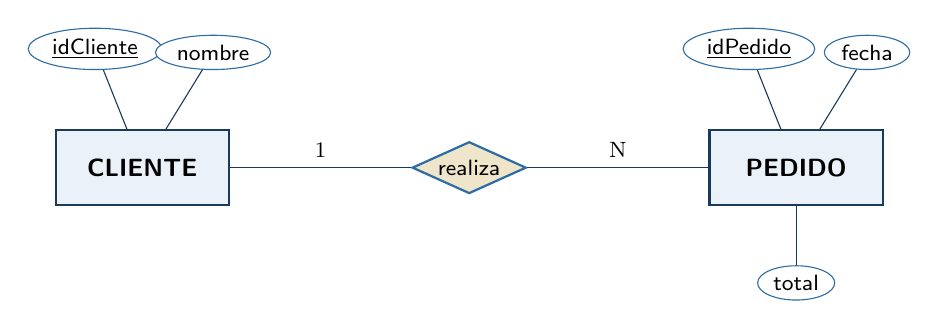
\begin{tikzpicture}[
			entidad/.style={draw=darkblue,thick,fill=softblue,minimum width=2.2cm,minimum height=0.95cm,font=\small\sffamily\bfseries},
			relacion/.style={draw=midblue,thick,fill=gold!30,diamond,aspect=2.2,inner sep=1pt,font=\footnotesize\sffamily},
			atrib/.style={draw=midblue,fill=white,ellipse,inner sep=1.6pt,font=\footnotesize\sffamily},
			link/.style={draw=darkblue}
			]
			\node[entidad] (cli) {CLIENTE};
			\node[relacion] (rel) [right=2.3cm of cli] {realiza};
			\node[entidad] (ped) [right=2.3cm of rel] {PEDIDO};
			\draw[link] (cli) -- node[above,font=\footnotesize]{1} (rel);
			\draw[link] (rel) -- node[above,font=\footnotesize]{N} (ped);
			\node[atrib] (a1) [above=0.75cm of cli,xshift=-0.6cm] {\underline{idCliente}};
			\node[atrib] (a2) [above=0.75cm of cli,xshift=0.9cm] {nombre};
			\node[atrib] (b1) [above=0.75cm of ped,xshift=-0.6cm] {\underline{idPedido}};
			\node[atrib] (b2) [above=0.75cm of ped,xshift=0.9cm] {fecha};
			\node[atrib] (b3) [below=0.75cm of ped] {total};
			\draw[link] (cli) -- (a1);
			\draw[link] (cli) -- (a2);
			\draw[link] (ped) -- (b1);
			\draw[link] (ped) -- (b2);
			\draw[link] (ped) -- (b3);
		\end{tikzpicture}
		\caption{Fragmento de modelo Entidad-Relaci\'on para un dominio de pedidos, con atributos clave subrayados y cardinalidad $1{:}N$.}
		\label{fig:er-ejemplo}
	\end{figure}
	
	El diagrama de clases del Lenguaje Unificado de Modelado (UML) generaliza al modelo ER al incorporar el comportamiento en la propia estructura. Seg\'un la especificaci\'on \textit{OMG UML} 2.5.1 \citep{omg_uml_2017}, cada clase se representa con un rect\'angulo dividido en tres compartimentos ---nombre, atributos y operaciones--- y las asociaciones se anotan con multiplicidades en sus extremos. La Figura~\ref{fig:clases-uml} traduce el modelo ER anterior a un diagrama de clases: las columnas de atributos preservan la informaci\'on del dominio, mientras que las operaciones a\~naden la sem\'antica funcional que el modelo ER no expresa. Esta equivalencia parcial es la que permite derivar esquemas de base de datos a partir de diagramas de clases y viceversa.
	
	\begin{figure}[htbp]
		\centering
		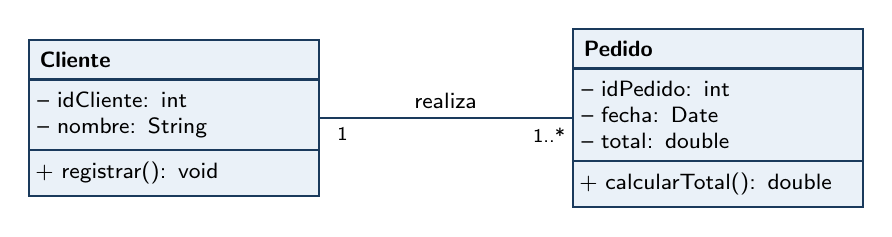
\begin{tikzpicture}[
			clase/.style={draw=darkblue,thick,fill=softblue,rectangle split,rectangle split parts=3,
				rectangle split part fill={softblue,white,white},text width=3.4cm,font=\footnotesize\sffamily,inner sep=4pt}
			]
			\node[clase] (cli) {
				{\bfseries\centering Cliente}
				\nodepart{second}\raggedright -- idCliente: int\\ -- nombre: String
				\nodepart{third}\raggedright + registrar(): void
			};
			\node[clase] (ped) [right=3.2cm of cli] {
				{\bfseries\centering Pedido}
				\nodepart{second}\raggedright -- idPedido: int\\ -- fecha: Date\\ -- total: double
				\nodepart{third}\raggedright + calcularTotal(): double
			};
			\draw[thick,darkblue] (cli.east) -- (ped.west);
			\path (cli.east) -- (ped.west)
			node[pos=0.5,above,font=\footnotesize\sffamily]{realiza}
			node[pos=0.09,below,font=\scriptsize\sffamily]{1}
			node[pos=0.91,below,font=\scriptsize\sffamily]{1..*};
		\end{tikzpicture}
		\caption{Diagrama de clases UML equivalente al modelo ER de la Figura~\ref{fig:er-ejemplo}; los compartimentos de operaciones a\~naden la sem\'antica funcional.}
		\label{fig:clases-uml}
	\end{figure}
	
	La elecci\'on entre ambas notaciones no es indiferente para la validaci\'on. El modelo ER favorece la revisi\'on con expertos del dominio poco familiarizados con la programaci\'on, porque su vocabulario es cercano al del negocio; el diagrama de clases, en cambio, facilita la verificaci\'on de consistencia con el dise\~no orientado a objetos y con las reglas de integridad. Wiegers y Beatty~\citep{wiegers_beatty_2013} recomiendan mantener ambos niveles sincronizados mediante un diccionario de datos \'unico, de modo que cada entidad, atributo y relaci\'on tenga una definici\'on textual precisa que sirva de referencia en las inspecciones.
	
	\subsection{Modelos funcionales: diagramas de flujo de datos, DFD esencial y actividades UML}
	
	La perspectiva funcional describe c\'omo el sistema transforma entradas en salidas mediante procesos que consumen y producen flujos de datos. El Diagrama de Flujo de Datos (DFD), formalizado en el an\'alisis estructurado de DeMarco~\citep{demarco_1979}, emplea cuatro s\'imbolos: procesos, flujos de datos, almacenes y entidades externas. La Figura~\ref{fig:dfd} presenta un DFD de nivel~1 para el registro de un pedido, donde el proceso \textsf{1.0 Registrar pedido} recibe los datos de la entidad externa \textsf{Cliente}, deja constancia en el almac\'en \textsf{D1 Pedidos} y devuelve una confirmaci\'on.
	
	\begin{figure}[htbp]
		\centering
		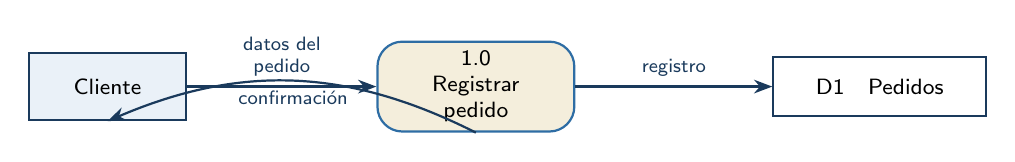
\begin{tikzpicture}[
			ext/.style={draw=darkblue,thick,fill=softblue,minimum width=2cm,minimum height=0.85cm,font=\footnotesize\sffamily},
			proc/.style={draw=midblue,thick,fill=gold!20,rounded corners=9pt,minimum width=2.5cm,minimum height=1.05cm,align=center,font=\footnotesize\sffamily},
			store/.style={draw=darkblue,thick,fill=white,minimum width=2.7cm,minimum height=0.75cm,font=\footnotesize\sffamily},
			flow/.style={-Stealth,thick,darkblue,font=\scriptsize\sffamily}
			]
			\node[ext] (cli) {Cliente};
			\node[proc] (p1) [right=2.4cm of cli] {1.0\\ Registrar\\ pedido};
			\node[store] (d1) [right=2.5cm of p1] {D1\quad Pedidos};
			\draw[flow] (cli) -- node[above,align=center]{datos del\\ pedido} (p1);
			\draw[flow] (p1) -- node[above]{registro} (d1);
			\draw[flow] (p1.south) to[bend right=25] node[below]{confirmaci\'on} (cli.south);
		\end{tikzpicture}
		\caption{Diagrama de Flujo de Datos de nivel~1 para el registro de un pedido; los almacenes se etiquetan con el prefijo \textsf{D}.}
		\label{fig:dfd}
	\end{figure}
	
	El DFD \textit{esencial} lleva esta abstracci\'on al l\'imite: describe la l\'ogica del sistema suponiendo una tecnolog\'ia perfecta ---procesadores infinitamente r\'apidos y memoria ilimitada---, de modo que quedan \'unicamente las transformaciones y los almacenes que el dominio exige, libres de detalles de implementaci\'on. Esta depuraci\'on es valiosa para la validaci\'on porque separa los requisitos esenciales de las decisiones de dise\~no, y permite preguntar a los interesados si la l\'ogica capturada es correcta con independencia de c\'omo se implemente. Pohl~\citep{pohl_2010} advierte, no obstante, que el DFD carece de una sem\'antica de control precisa, por lo que debe complementarse con modelos de comportamiento.
	
	El diagrama de actividades UML es la notaci\'on moderna que subsana esa carencia, al integrar flujo de control y flujo de datos con soporte expl\'icito para decisiones, bifurcaciones, concurrencia y carriles de responsabilidad. La Figura~\ref{fig:actividad} modela el mismo proceso de pedido incorporando una decisi\'on sobre la disponibilidad de \textit{stock}, con dos caminos alternativos que convergen en un nodo final. Frente al DFD, el diagrama de actividades expresa el orden temporal de las acciones, lo que facilita validar reglas de negocio como ``no se confirma un pedido sin verificar existencias''.
	
	\begin{figure}[htbp]
		\centering
		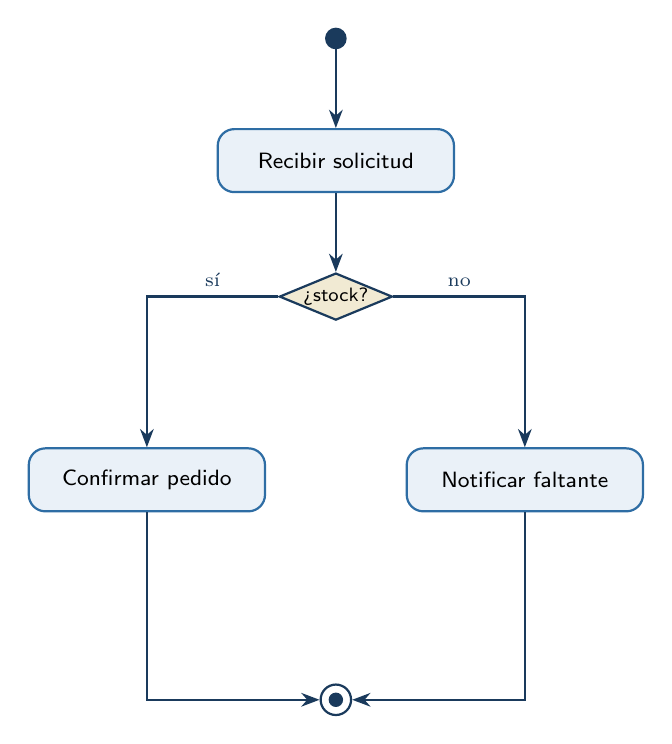
\begin{tikzpicture}[
			node distance=1.0cm,
			accion/.style={draw=midblue,thick,fill=softblue,rounded corners=6pt,minimum width=3cm,minimum height=0.8cm,align=center,font=\footnotesize\sffamily},
			dec/.style={draw=darkblue,thick,fill=gold!25,diamond,aspect=2.4,inner sep=0pt,font=\scriptsize\sffamily},
			ini/.style={circle,draw=darkblue,thick,fill=darkblue,minimum size=7pt,inner sep=0pt},
			arr/.style={-Stealth,thick,darkblue,font=\scriptsize\sffamily}
			]
			\node[ini] (ini) {};
			\node[accion] (a1) [below=of ini] {Recibir solicitud};
			\node[dec] (d1) [below=of a1] {\,¿stock?\,};
			\node[accion] (a2) [below=1.6cm of d1,xshift=-2.4cm] {Confirmar pedido};
			\node[accion] (a3) [below=1.6cm of d1,xshift=2.4cm] {Notificar faltante};
			\node[circle,draw=darkblue,thick,minimum size=11pt,inner sep=0pt] (fin) [below=4.6cm of d1] {};
			\fill[darkblue] (fin) circle (2.6pt);
			\draw[arr] (ini)--(a1);
			\draw[arr] (a1)--(d1);
			\draw[arr] (d1) -| node[pos=0.25,above,font=\scriptsize]{s\'i} (a2);
			\draw[arr] (d1) -| node[pos=0.25,above,font=\scriptsize]{no} (a3);
			\draw[arr] (a2) |- (fin);
			\draw[arr] (a3) |- (fin);
		\end{tikzpicture}
		\caption{Diagrama de actividades UML del registro de un pedido; la decisi\'on ¿stock? gobierna dos caminos que convergen en el nodo final.}
		\label{fig:actividad}
	\end{figure}
	
	\subsection{Modelos de comportamiento: aut\'omatas finitos, statecharts y m\'aquinas de estado UML}
	
	La perspectiva de comportamiento describe c\'omo cambia el estado del sistema ---o de una entidad relevante--- en respuesta a los eventos que recibe. El aut\'omata finito es el modelo b\'asico: un conjunto finito de estados, un estado inicial, transiciones etiquetadas con eventos y, en su versi\'on reconocedora, uno o m\'as estados de aceptaci\'on. La Figura~\ref{fig:estados} modela el ciclo de vida de un \textsf{Pedido} como una m\'aquina de estados UML, notaci\'on que hereda del aut\'omata finito pero admite condiciones de guarda, acciones de entrada/salida y estados compuestos.
	
	\begin{figure}[htbp]
		\centering
		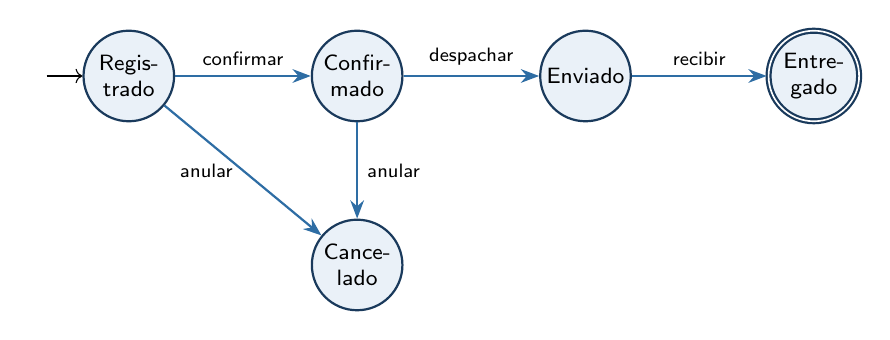
\begin{tikzpicture}[
			node distance=2.8cm and 2.9cm, on grid,
			every state/.style={draw=darkblue,thick,fill=softblue,font=\footnotesize\sffamily,minimum size=1.15cm,inner sep=1pt,align=center},
			arr/.style={draw=midblue,thick,font=\scriptsize\sffamily}
			]
			\node[state,initial,initial text=] (s0) {Regis-\\trado};
			\node[state] (s1) [right=of s0] {Confir-\\mado};
			\node[state] (s2) [right=of s1] {Enviado};
			\node[state,accepting] (s3) [right=of s2] {Entre-\\gado};
			\node[state] (sc) [below=2.4cm of s1] {Cance-\\lado};
			\path[->,>=Stealth]
			(s0) edge[arr] node[above]{confirmar} (s1)
			(s1) edge[arr] node[above]{despachar} (s2)
			(s2) edge[arr] node[above]{recibir} (s3)
			(s0) edge[arr,swap] node[left]{anular} (sc)
			(s1) edge[arr] node[right]{anular} (sc);
		\end{tikzpicture}
		\caption{M\'aquina de estados UML del ciclo de vida de un pedido; \textsf{Entregado} es el estado final de aceptaci\'on.}
		\label{fig:estados}
	\end{figure}
	
	Cuando el n\'umero de estados crece, el aut\'omata plano se vuelve inmanejable. Los \textit{statecharts} de Harel~\citep{harel_1987} introducen tres mecanismos que dominan esa complejidad: la jerarqu\'ia (un superestado agrupa subestados y factoriza las transiciones comunes), la ortogonalidad (regiones concurrentes que describen comportamiento paralelo) y la memoria de historia. La Figura~\ref{fig:statechart} ilustra la jerarqu\'ia: el superestado \textsf{Activo} agrupa a \textsf{Confirmado} y \textsf{Enviado}, de modo que la transici\'on \textsf{anular} se define una sola vez a nivel del superestado en lugar de repetirse en cada subestado. UML adopt\'o directamente este formalismo en sus m\'aquinas de estado, lo que convierte a los statecharts en el sustrato te\'orico de la notaci\'on de comportamiento m\'as usada en la industria.
	
	\begin{figure}[htbp]
		\centering
		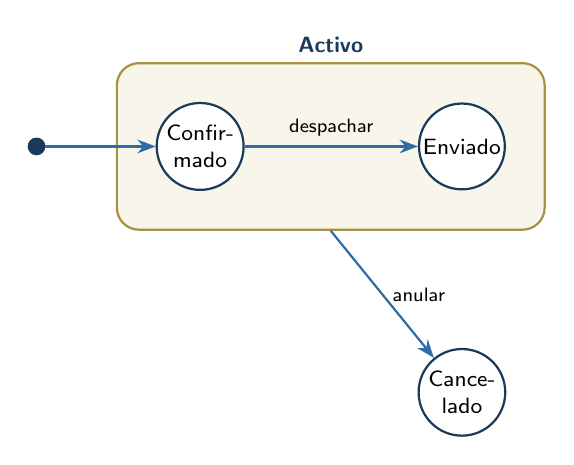
\begin{tikzpicture}[
			every state/.style={draw=darkblue,thick,fill=white,font=\footnotesize\sffamily,minimum size=1.0cm,inner sep=1pt,align=center},
			arr/.style={-Stealth,draw=midblue,thick,font=\scriptsize\sffamily}
			]
			\node[state] (c) {Confir-\\mado};
			\node[state] (e) [right=2.2cm of c] {Enviado};
			\begin{scope}[on background layer]
				\node[draw=gold!85!black,thick,fill=gold!12,rounded corners=8pt,fit=(c)(e),
				inner sep=14pt,label={[font=\footnotesize\sffamily\bfseries,text=darkblue]above:Activo}] (sup) {};
			\end{scope}
			\node[circle,draw=darkblue,fill=darkblue,minimum size=6pt,inner sep=0pt] (ini) [left=1.4cm of c] {};
			\node[state] (canc) [below=2.0cm of e] {Cance-\\lado};
			\draw[arr] (ini) -- (c);
			\draw[arr] (c) -- node[above]{despachar} (e);
			\draw[arr] (sup.south) -- node[right]{anular} (canc);
		\end{tikzpicture}
		\caption{Statechart con jerarqu\'ia: el superestado \textsf{Activo} factoriza la transici\'on \textsf{anular} de sus subestados.}
		\label{fig:statechart}
	\end{figure}
	
	\subsection{Interrelaciones entre las tres perspectivas: datos, funci\'on y comportamiento}
	
	Ninguna de las tres perspectivas basta por s\'i sola para especificar un sistema no trivial, porque cada una silencia informaci\'on que las otras hacen expl\'icita. El modelo de datos ignora el orden temporal; el modelo funcional no fija el ciclo de vida de las entidades; el modelo de comportamiento presupone unos datos y unas funciones que no define. La Figura~\ref{fig:perspectivas} representa esta complementariedad como un tri\'angulo cuyos v\'ertices se conectan mediante relaciones de consistencia que la validaci\'on debe verificar de forma cruzada.
	
	\begin{figure}[htbp]
		\centering
		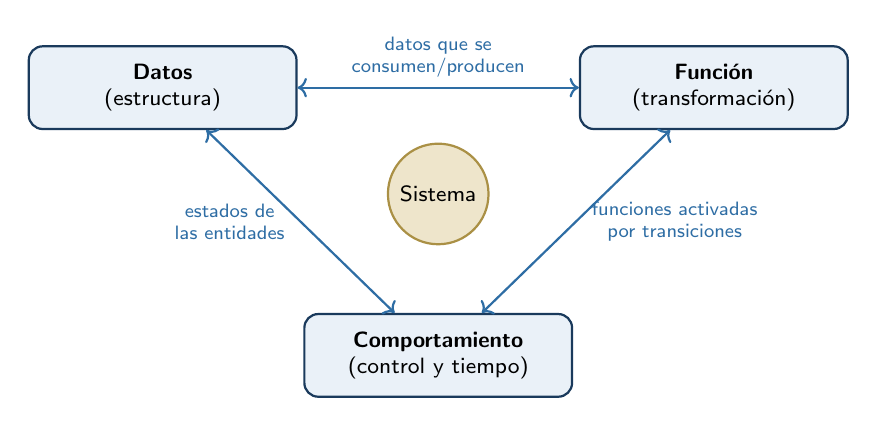
\begin{tikzpicture}[
			persp/.style={draw=darkblue,thick,fill=softblue,rounded corners=5pt,minimum width=3.4cm,minimum height=1.05cm,align=center,font=\footnotesize\sffamily\bfseries},
			rel/.style={midblue,font=\scriptsize\sffamily,align=center}
			]
			\node[persp] (dat) at (0,0) {Datos\\{\footnotesize\mdseries(estructura)}};
			\node[persp] (fun) at (7,0) {Funci\'on\\{\footnotesize\mdseries(transformaci\'on)}};
			\node[persp] (comp) at (3.5,-3.4) {Comportamiento\\{\footnotesize\mdseries(control y tiempo)}};
			\node[circle,draw=gold!85!black,fill=gold!30,thick,font=\footnotesize\sffamily] (sis) at (3.5,-1.35) {Sistema};
			\draw[<->,thick,midblue] (dat) -- node[above,rel]{datos que se\\ consumen/producen} (fun);
			\draw[<->,thick,midblue] (fun) -- node[right,rel,xshift=2pt]{funciones activadas\\ por transiciones} (comp);
			\draw[<->,thick,midblue] (dat) -- node[left,rel,xshift=-2pt]{estados de\\ las entidades} (comp);
		\end{tikzpicture}
		\caption{Complementariedad de las tres perspectivas; las aristas indican las relaciones de consistencia que la validaci\'on verifica de forma cruzada.}
		\label{fig:perspectivas}
	\end{figure}
	
	La consistencia entre perspectivas es una fuente sistem\'atica de defectos que las inspecciones deben rastrear. Un evento que aparece en la m\'aquina de estados debe corresponder a alguna funci\'on del modelo funcional; toda entidad citada por una funci\'on debe existir en el modelo de datos; y cada atributo modificable debe tener asociado alg\'un cambio de estado observable cuando el dominio as\'i lo exige. La revisi\'on sistem\'atica de Zhao y Zhou~\citep{zhao_mbre_2026} sobre ingenier\'ia de requisitos basada en modelos documenta que la mayor\'ia de las t\'ecnicas maduras persiguen precisamente esta integraci\'on, y que las herramientas de transformaci\'on de modelos permiten hoy verificar automatizadamente varias de estas reglas de correspondencia.
	
	Desde la \'optica de la calidad, esta triangulaci\'on es una forma econ\'omica de validaci\'on: al contrastar cada perspectiva con las otras dos se detectan omisiones y contradicciones que una lectura aislada no revelar\'ia, en aplicaci\'on directa del principio de validaci\'on desde distintas vistas que se formaliza en la secci\'on siguiente. La norma \textit{ISO/IEC/IEEE} 29148 \citep{iso29148_2018} refuerza esta idea al exigir que el conjunto de requisitos sea internamente consistente, propiedad que solo puede comprobarse examinando las relaciones entre los modelos y no cada modelo por separado.
	
	% #####################################################################
	\section{Gesti\'on de Requisitos}
	
	Comprobar que los modelos anteriores describen el sistema correcto exige una disciplina propia, con motivaci\'on, principios y t\'ecnicas diferenciadas. La validaci\'on de requisitos es la actividad que examina los artefactos de requisitos para descubrir defectos antes de que se propaguen al dise\~no y a la codificaci\'on, donde corregirlos cuesta \'ordenes de magnitud m\'as \citep{pohl_2010,sommerville_2016}. Las cuatro subsecciones siguientes recorren su fundamento ---los principios y el aseguramiento de la calidad---, las t\'ecnicas de evaluaci\'on basadas en lectura humana, el uso de prototipos y la validaci\'on de modelos, metas y escenarios, y finalmente las pruebas de aceptaci\'on como puente hacia la verificaci\'on del producto.
	
	\subsection{Motivaci\'on y seis principios de validaci\'on. Aseguramiento de la calidad en IR}
	
	La motivaci\'on de la validaci\'on es econ\'omica y a la vez t\'ecnica: un requisito err\'oneo que sobrevive hasta la fase de pruebas puede costar hasta cien veces m\'as que si se hubiera detectado durante la elicitaci\'on \citep{sommerville_2016}. El aseguramiento de la calidad en ingenier\'ia de requisitos verifica tres aspectos complementarios que Pohl~\citep{pohl_2010} denomina las tres dimensiones de calidad: el \textit{contenido} (que todos los requisitos relevantes est\'en presentes y sean correctos), la \textit{documentaci\'on} (que se ajusten a las reglas de formato y estilo acordadas) y el \textit{acuerdo} (que los interesados hayan consensuado cada requisito). La Figura~\ref{fig:calidad} representa estas tres dimensiones y su intersecci\'on, que corresponde a un requisito plenamente validado.
	
	\begin{figure}[htbp]
		\centering
		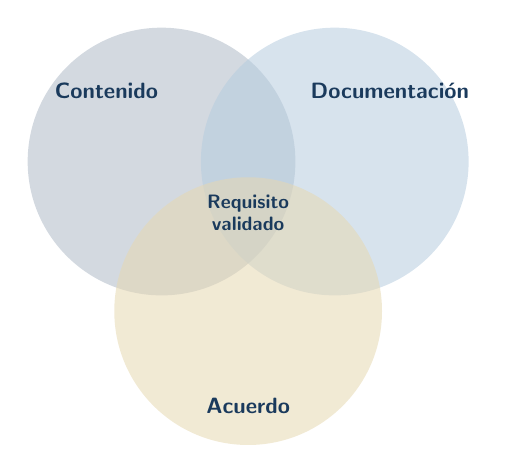
\begin{tikzpicture}[font=\footnotesize\sffamily]
			\begin{scope}[opacity=0.55,text opacity=1]
				\fill[darkblue!35] (0,0) circle (1.7cm);
				\fill[midblue!35] (2.2,0) circle (1.7cm);
				\fill[gold!45] (1.1,-1.9) circle (1.7cm);
			\end{scope}
			\node[text=darkblue,font=\footnotesize\sffamily\bfseries] at (-0.7,0.9) {Contenido};
			\node[text=darkblue,font=\footnotesize\sffamily\bfseries] at (2.9,0.9) {Documentaci\'on};
			\node[text=darkblue,font=\footnotesize\sffamily\bfseries] at (1.1,-3.1) {Acuerdo};
			\node[align=center,font=\scriptsize\sffamily\bfseries,text=darkblue] at (1.1,-0.65) {Requisito\\ validado};
		\end{tikzpicture}
		\caption{Las tres dimensiones de calidad del aseguramiento en IR; su intersecci\'on define un requisito validado.}
		\label{fig:calidad}
	\end{figure}
	
	Sobre esa base, Pohl~\citep{pohl_2010} formula seis principios que gu\'ian toda actividad de validaci\'on con independencia de la t\'ecnica empleada. La Tabla~\ref{tab:principios} los resume. El segundo principio ---separar la identificaci\'on de la correcci\'on--- es especialmente relevante en la pr\'actica, porque mezclar ambas actividades en una misma reuni\'on desv\'ia la atenci\'on hacia la discusi\'on de soluciones y reduce la tasa de defectos detectados; por ello las inspecciones formales prohiben expl\'icitamente proponer correcciones durante la sesi\'on de detecci\'on.
	
	\begin{table}[htbp]
		\centering
		\caption{Los seis principios de validaci\'on de requisitos seg\'un Pohl~\citep{pohl_2010}.}
		\label{tab:principios}
		\small\sffamily
		\begin{tabularx}{\linewidth}{@{}C{0.7cm} L{4.1cm} X@{}}
			\toprule
			\hd{N\textsuperscript{o}} & \hd{Principio} & \hd{Idea central}\\
			\midrule
			1 & Involucrar a los interesados correctos & Solo quien posee el conocimiento del dominio puede juzgar si un requisito es correcto.\\
			\rowcolor{rowgray}
			2 & Separar identificaci\'on y correcci\'on de errores & Detectar defectos y corregirlos son actividades distintas; mezclarlas reduce la eficacia.\\
			3 & Validar desde distintas vistas & Contrastar el mismo requisito bajo perspectivas de datos, funci\'on y comportamiento revela inconsistencias.\\
			\rowcolor{rowgray}
			4 & Cambiar de tipo de documentaci\'on & Reexpresar un requisito en otra representaci\'on (texto a modelo, o viceversa) expone ambig\"uedades ocultas.\\
			5 & Construir artefactos de desarrollo & Prototipos y modelos ejecutables hacen tangibles los defectos que el texto oculta.\\
			\rowcolor{rowgray}
			6 & Validar de forma repetida & La validaci\'on no es un hito \'unico sino una actividad recurrente a lo largo del proceso.\\
			\bottomrule
		\end{tabularx}
	\end{table}
	
	El aseguramiento de la calidad moderno complementa estos principios con apoyo automatizado. La revisi\'on sistem\'atica de Cheng et al.~\citep{cheng_genai_re_2026} documenta que los modelos de lenguaje de gran tama\~no ya se aplican con resultados prometedores a la detecci\'on de ambig\"uedad, la comprobaci\'on de completitud y la generaci\'on de preguntas de validaci\'on, aunque advierte que su salida requiere supervisi\'on humana porque puede introducir afirmaciones plausibles pero incorrectas. Esta cautela es coherente con el primer principio: la responsabilidad de juzgar la correcci\'on sigue recayendo en los interesados y el equipo, no en la herramienta.
	
	\subsection{Evaluaci\'on de requisitos: revisiones informales, walkthroughs e inspecciones formales (Fagan)}
	
	Las t\'ecnicas de evaluaci\'on basadas en lectura humana forman un continuo de formalidad creciente. La \textit{revisi\'on informal} consiste en que uno o m\'as colegas comenten un documento sin procedimiento predefinido; es barata y \'util en etapas tempranas, pero su cobertura es irregular. El \textit{walkthrough} a\~nade estructura: el autor gu\'ia a los participantes a trav\'es del artefacto para recoger observaciones, aunque conserva un car\'acter formativo y poco medido. La \textit{inspecci\'on formal} de Fagan~\citep{fagan_1976} es el extremo riguroso del continuo, con roles definidos, criterios de entrada y salida, y recolecci\'on de m\'etricas de defectos. La Tabla~\ref{tab:evaluacion} contrasta las tres t\'ecnicas.
	
	\begin{table}[htbp]
		\centering
		\caption{Comparaci\'on de las t\'ecnicas de evaluaci\'on de requisitos por lectura.}
		\label{tab:evaluacion}
		\small\sffamily
		\begin{tabularx}{\linewidth}{@{}L{3.0cm} X X X@{}}
			\toprule
			\hd{Criterio} & \hd{Revisi\'on informal} & \hd{Walkthrough} & \hd{Inspecci\'on (Fagan)}\\
			\midrule
			Formalidad & Baja & Media & Alta\\
			\rowcolor{rowgray}
			Roles definidos & No & Parcial (autor gu\'ia) & S\'i (moderador, autor, lector, inspectores, registrador)\\
			Criterios de entrada/salida & No & No & S\'i\\
			\rowcolor{rowgray}
			M\'etricas de defectos & No & Ocasional & S\'i, sistem\'aticas\\
			Costo relativo & Bajo & Medio & Alto\\
			\bottomrule
		\end{tabularx}
	\end{table}
	
	La inspecci\'on de Fagan se organiza en seis fases encadenadas que la Figura~\ref{fig:fagan} representa. Tras la \textit{planificaci\'on} (seleccionar el material y el equipo) y una \textit{visi\'on general} opcional que nivela el conocimiento, cada inspector realiza una \textit{preparaci\'on} individual buscando defectos; la \textit{reuni\'on de inspecci\'on} los registra sin corregirlos ---en aplicaci\'on del segundo principio de validaci\'on---; el autor ejecuta el \textit{retrabajo}; y el moderador comprueba en el \textit{seguimiento} que todo defecto se haya resuelto, decidiendo si el artefacto pasa o debe reinspeccionarse.
	
	\begin{figure}[htbp]
		\centering
		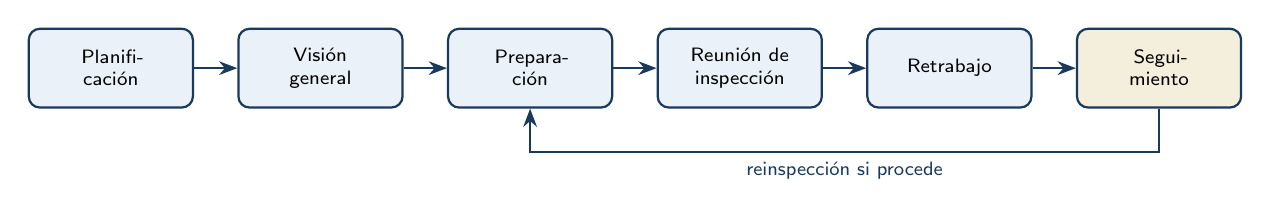
\begin{tikzpicture}[
			node distance=0.55cm,
			fase/.style={draw=darkblue,thick,fill=softblue,rounded corners=4pt,minimum height=1.0cm,text width=1.85cm,align=center,font=\scriptsize\sffamily},
			arr/.style={-Stealth,thick,darkblue}
			]
			\node[fase] (f1) {Planifi-\\caci\'on};
			\node[fase] (f2) [right=of f1] {Visi\'on\\ general};
			\node[fase] (f3) [right=of f2] {Prepara-\\ci\'on};
			\node[fase] (f4) [right=of f3] {Reuni\'on de\\ inspecci\'on};
			\node[fase] (f5) [right=of f4] {Retrabajo};
			\node[fase,fill=gold!20] (f6) [right=of f5] {Segui-\\miento};
			\draw[arr] (f1)--(f2);
			\draw[arr] (f2)--(f3);
			\draw[arr] (f3)--(f4);
			\draw[arr] (f4)--(f5);
			\draw[arr] (f5)--(f6);
			\draw[arr] (f6.south) -- ++(0,-0.55) -| node[pos=0.25,below,font=\scriptsize\sffamily]{reinspecci\'on si procede} (f3.south);
		\end{tikzpicture}
		\caption{Las seis fases de la inspecci\'on formal de Fagan~\citep{fagan_1976}; el seguimiento puede reactivar la preparaci\'on.}
		\label{fig:fagan}
	\end{figure}
	
	La evidencia acumulada muestra que las inspecciones formales son una de las t\'ecnicas de aseguramiento de la calidad con mejor relaci\'on costo-beneficio, capaces de eliminar una fracci\'on elevada de los defectos antes de la codificaci\'on \citep{sommerville_2016}. Su limitaci\'on es el esfuerzo que demandan, por lo que en la pr\'actica se reservan para los artefactos de mayor riesgo ---requisitos cr\'iticos de seguridad o de alto impacto contractual--- y se combinan con revisiones m\'as ligeras para el resto del documento.
	
	\subsection{Prototipos como t\'ecnica de validaci\'on. Validaci\'on del modelo. Validaci\'on de metas y escenarios}
	
	El quinto principio de validaci\'on ---construir artefactos de desarrollo--- encuentra su expresi\'on m\'as directa en el prototipado. Un prototipo hace tangible una parte del sistema y permite que los interesados reaccionen ante algo concreto, revelando necesidades latentes que ninguna lectura de texto habr\'ia expuesto. La Figura~\ref{fig:prototipos} organiza los prototipos seg\'un tres criterios que Pohl~\citep{pohl_2010} y Sommerville~\citep{sommerville_2016} distinguen: el objetivo, el alcance y el destino final del artefacto.
	
	\begin{figure}[htbp]
		\centering
		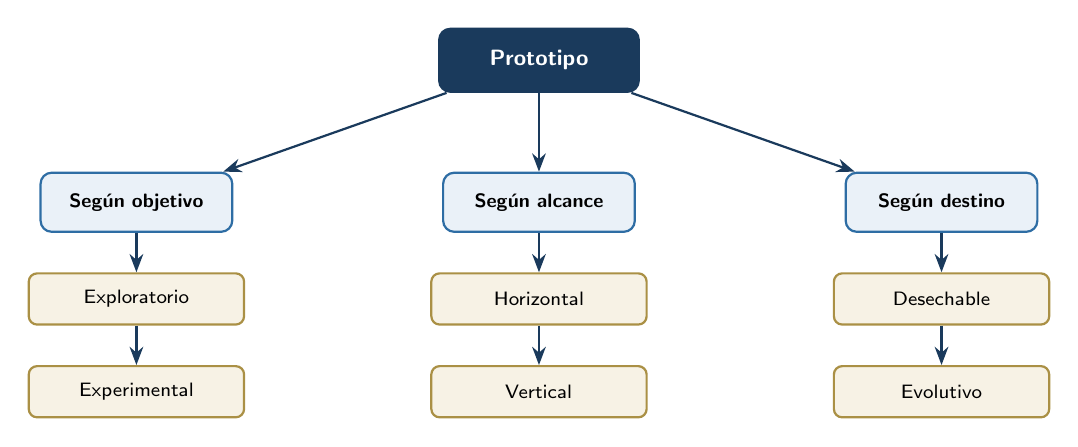
\begin{tikzpicture}[
			node distance=0.5cm and 0.9cm,
			raiz/.style={draw=darkblue,thick,fill=darkblue,text=white,rounded corners=4pt,minimum height=0.8cm,text width=2.3cm,align=center,font=\footnotesize\sffamily\bfseries},
			crit/.style={draw=midblue,thick,fill=softblue,rounded corners=4pt,minimum height=0.75cm,text width=2.2cm,align=center,font=\scriptsize\sffamily\bfseries},
			hoja/.style={draw=gold!85!black,thick,fill=gold!15,rounded corners=3pt,minimum height=0.65cm,text width=2.5cm,align=center,font=\scriptsize\sffamily},
			arr/.style={-Stealth,thick,darkblue}
			]
			\node[raiz] (r) {Prototipo};
			\node[crit] (obj) [below left=1.0cm and 2.6cm of r] {Seg\'un objetivo};
			\node[crit] (alc) [below=1.0cm of r] {Seg\'un alcance};
			\node[crit] (des) [below right=1.0cm and 2.6cm of r] {Seg\'un destino};
			\node[hoja] (o1) [below=of obj] {Exploratorio};
			\node[hoja] (o2) [below=of o1] {Experimental};
			\node[hoja] (a1) [below=of alc] {Horizontal};
			\node[hoja] (a2) [below=of a1] {Vertical};
			\node[hoja] (d1) [below=of des] {Desechable};
			\node[hoja] (d2) [below=of d1] {Evolutivo};
			\draw[arr] (r)--(obj); \draw[arr] (r)--(alc); \draw[arr] (r)--(des);
			\draw[arr] (obj)--(o1); \draw[arr] (o1)--(o2);
			\draw[arr] (alc)--(a1); \draw[arr] (a1)--(a2);
			\draw[arr] (des)--(d1); \draw[arr] (d1)--(d2);
		\end{tikzpicture}
		\caption{Clasificaci\'on de prototipos seg\'un objetivo, alcance y destino, usados como t\'ecnica de validaci\'on.}
		\label{fig:prototipos}
	\end{figure}
	
	M\'as all\'a del prototipo, la validaci\'on del modelo comprueba que los diagramas producidos en la Secci\'on~4.1 sean correctos respecto de la realidad que pretenden describir, y consistentes entre s\'i. Aqu\'i el cuarto principio ---cambiar de tipo de documentaci\'on--- resulta decisivo: traducir un requisito textual a una m\'aquina de estados obliga a explicitar el estado inicial, las transiciones y las condiciones de guarda, y en ese proceso afloran huecos que el enunciado en prosa toleraba. Recorrer la m\'aquina de estados de la Figura~\ref{fig:estados} junto a un experto del dominio es, en s\'i mismo, un acto de validaci\'on.
	
	La validaci\'on de metas y escenarios cierra el cuadro comprobando que la soluci\'on especificada satisface las intenciones de alto nivel de los interesados. Se verifica que cada meta se descomponga en subrequisitos que efectivamente la realizan, y que los escenarios ---casos de uso o historias de usuario--- cubran tanto los caminos normales como las excepciones relevantes. Wiegers y Beatty~\citep{wiegers_beatty_2013} recomiendan derivar de cada escenario un conjunto de condiciones observables que servir\'an, m\'as adelante, como base de las pruebas de aceptaci\'on, enlazando as\'i la validaci\'on de requisitos con la verificaci\'on del producto terminado.
	
	\subsection{Pruebas de aceptaci\'on: definici\'on, tipos (funcional, no funcional, regresi\'on) y relaci\'on con requisitos}
	
	La prueba de aceptaci\'on es la comprobaci\'on formal, ejecutada con la participaci\'on o en representaci\'on del cliente, de que el sistema entregado satisface los requisitos acordados y es apto para su uso. Se distingue de la verificaci\'on interna en su prop\'osito y en su audiencia: no busca defectos de implementaci\'on sino evidencia de que el producto correcto fue construido, y su criterio de \'exito son los requisitos, no el dise\~no. Por ello cada prueba de aceptaci\'on debe trazar a uno o m\'as requisitos, como ilustra la Figura~\ref{fig:aceptacion}, y un requisito sin prueba asociada es una se\~nal de requisito no verificable ---defecto que la norma \textit{ISO/IEC/IEEE} 29148 clasifica como violaci\'on de la propiedad de verificabilidad \citep{iso29148_2018}.
	
	\begin{figure}[htbp]
		\centering
		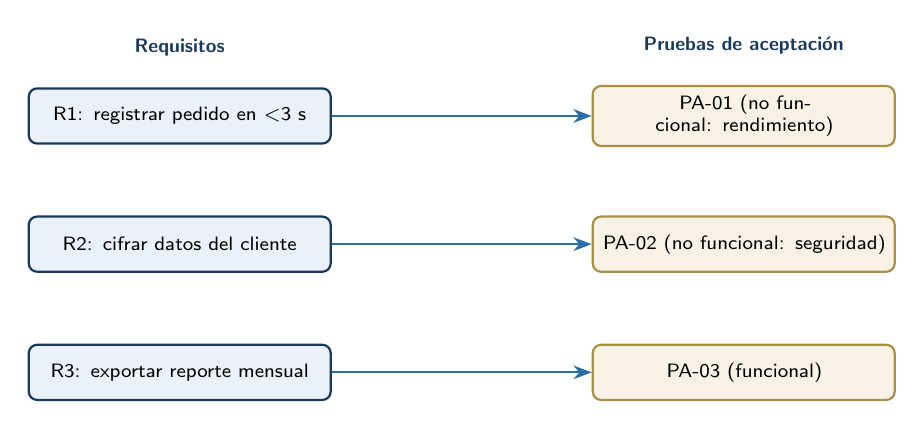
\begin{tikzpicture}[
			node distance=0.9cm,
			req/.style={draw=darkblue,thick,fill=softblue,rounded corners=3pt,minimum height=0.7cm,text width=3.6cm,align=center,font=\scriptsize\sffamily},
			pru/.style={draw=gold!85!black,thick,fill=gold!15,rounded corners=3pt,minimum height=0.7cm,text width=3.6cm,align=center,font=\scriptsize\sffamily},
			arr/.style={-Stealth,thick,midblue}
			]
			\node[req] (r1) {R1: registrar pedido en $<$3 s};
			\node[req] (r2) [below=of r1] {R2: cifrar datos del cliente};
			\node[req] (r3) [below=of r2] {R3: exportar reporte mensual};
			\node[pru] (t1) [right=3.3cm of r1] {PA-01 (no funcional: rendimiento)};
			\node[pru] (t2) [right=3.3cm of r2] {PA-02 (no funcional: seguridad)};
			\node[pru] (t3) [right=3.3cm of r3] {PA-03 (funcional)};
			\draw[arr] (r1)--(t1);
			\draw[arr] (r2)--(t2);
			\draw[arr] (r3)--(t3);
			\node[font=\scriptsize\sffamily\bfseries,text=darkblue] at ($(r1.north)+(0,0.5)$) {Requisitos};
			\node[font=\scriptsize\sffamily\bfseries,text=darkblue] at ($(t1.north)+(0,0.5)$) {Pruebas de aceptaci\'on};
		\end{tikzpicture}
		\caption{Cada prueba de aceptaci\'on traza al menos a un requisito; la ausencia de traza delata un requisito no verificable.}
		\label{fig:aceptacion}
	\end{figure}
	
	Seg\'un el atributo de calidad que examinan, las pruebas de aceptaci\'on se agrupan en tres tipos. Las \textit{funcionales} comprueban que el sistema produce las salidas correctas ante entradas dadas, es decir, que cumple los requisitos funcionales. Las \textit{no funcionales} verifican atributos como rendimiento, seguridad, usabilidad o fiabilidad, en correspondencia con las caracter\'isticas del modelo de calidad de producto \textit{ISO/IEC} 25010 \citep{iso25010_2023}. Las de \textit{regresi\'on} reejecutan pruebas previamente superadas tras un cambio, para asegurar que la nueva versi\'on no rompi\'o funcionalidad ya aceptada; su papel es central en la gesti\'on de cambios que se aborda en la secci\'on siguiente, pues cada modificaci\'on de un requisito obliga a revalidar los requisitos dependientes.
	
	El aseguramiento de la trazabilidad entre requisitos y pruebas de aceptaci\'on es, en consecuencia, un requisito de gesti\'on y no meramente de prueba. La gu\'ia SWEBOK v4 \citep{swebok_v4_2024} sit\'ua la definici\'on de criterios de aceptaci\'on dentro de las buenas pr\'acticas de la ingenier\'ia de requisitos, precisamente porque son el instrumento que hace operativa la propiedad de verificabilidad y conecta la validaci\'on temprana con la aceptaci\'on final del producto.
	
	% #####################################################################
	\section{Herramientas, Est\'andares e IR \'Agil}
	
	Validar los requisitos una vez no basta: el contexto de un proyecto cambia, los interesados revisan sus necesidades y los artefactos deben mantenerse coherentes mientras evolucionan. La gesti\'on de requisitos es la actividad transversal que preserva esa coherencia a lo largo del tiempo, controlando la naturaleza iterativa del proceso, los cambios, la trazabilidad y la configuraci\'on de los artefactos \citep{pohl_2010,iso29148_2018}. Las cuatro subsecciones siguientes desarrollan estos pilares, que constituyen la base sobre la que operan las herramientas CASE y los est\'andares tratados en la \'ultima secci\'on del cap\'itulo.
	
	\subsection{Naturaleza iterativa del proceso de IR. Gesti\'on del contexto y de actividades de IR}
	
	La ingenier\'ia de requisitos no es una fase que concluye antes del dise\~no, sino un proceso iterativo cuyas actividades se entrelazan y se repiten a medida que crece el conocimiento del problema. Pohl~\citep{pohl_2010} organiza este proceso en tres actividades centrales ---elicitaci\'on, documentaci\'on y negociaci\'on--- y dos actividades transversales ---validaci\'on y gesti\'on--- que act\'uan de forma continua sobre las primeras. La Figura~\ref{fig:iterativo} representa esta estructura: las actividades centrales forman un ciclo que se recorre tantas veces como sea necesario, mientras que la validaci\'on y la gesti\'on lo envuelven de manera permanente.
	
	\begin{figure}[htbp]
		\centering
		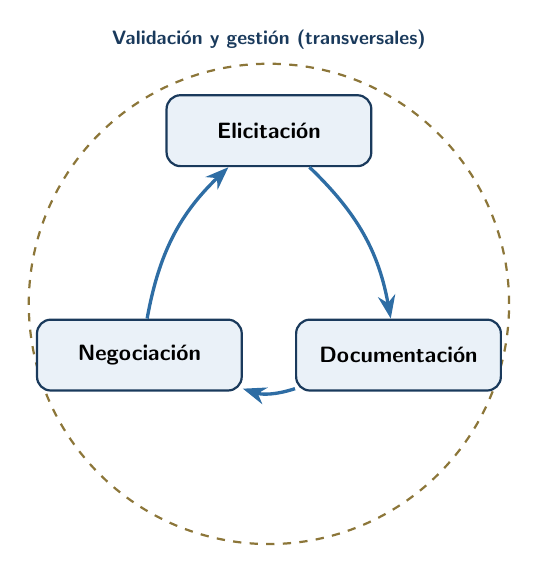
\begin{tikzpicture}[
			act/.style={draw=darkblue,thick,fill=softblue,rounded corners=5pt,minimum width=2.6cm,minimum height=0.9cm,align=center,font=\footnotesize\sffamily\bfseries},
			arr/.style={-Stealth,very thick,midblue}
			]
			\begin{scope}[on background layer]
				\draw[gold!70!black,dashed,thick] (0,-0.3) circle (3.05cm);
				\node[font=\scriptsize\sffamily\bfseries,text=darkblue,fill=white,inner sep=1pt] at (90:3.05) {Validaci\'on y gesti\'on (transversales)};
			\end{scope}
			\node[act] (e) at (90:1.9) {Elicitaci\'on};
			\node[act] (d) at (330:1.9) {Documentaci\'on};
			\node[act] (n) at (210:1.9) {Negociaci\'on};
			\draw[arr] (e) to[bend left=18] (d);
			\draw[arr] (d) to[bend left=18] (n);
			\draw[arr] (n) to[bend left=18] (e);
		\end{tikzpicture}
		\caption{Naturaleza iterativa del proceso de IR: las tres actividades centrales forman un ciclo envuelto por la validaci\'on y la gesti\'on.}
		\label{fig:iterativo}
	\end{figure}
	
	Gestionar este proceso implica gestionar tambi\'en el contexto que lo rodea. El l\'imite del sistema, los interesados, las normas aplicables y las decisiones ya tomadas conforman un contexto que no es est\'atico: un cambio regulatorio o la incorporaci\'on de un nuevo interesado pueden invalidar requisitos que se cre\'ian estables. Por ello la gesti\'on de actividades de IR planifica qu\'e t\'ecnicas aplicar en cada iteraci\'on, asigna responsabilidades y decide cu\'ando un artefacto est\'a suficientemente maduro para congelarse en una l\'inea base. Hoy y Xu~\citep{hoy_agile_re_2023} muestran, en su revisi\'on sistem\'atica sobre IR \'agil, que esta gesti\'on iterativa del contexto es precisamente el punto donde los enfoques \'agiles aportan mayor valor, al reemplazar la especificaci\'on exhaustiva inicial por refinamientos sucesivos guiados por la retroalimentaci\'on.
	
	\subsection{Gesti\'on del cambio: Change Control Board, documentaci\'on de cambios y proceso de cambio}
	
	Todo requisito consolidado en una l\'inea base queda protegido por un proceso de control de cambios que impide modificaciones arbitrarias y garantiza que cada alteraci\'on sea evaluada, aprobada y documentada. El \'organo responsable de esas decisiones es el \textit{Change Control Board} (CCB), un comit\'e que re\'une a representantes de los interesados, del equipo t\'ecnico y de la gesti\'on del proyecto, con autoridad para aprobar, rechazar o diferir cada solicitud de cambio \citep{wiegers_beatty_2013}. La Figura~\ref{fig:cambio} describe el flujo t\'ipico de una solicitud de cambio desde su registro hasta su cierre.
	
	\begin{figure}[htbp]
		\centering
		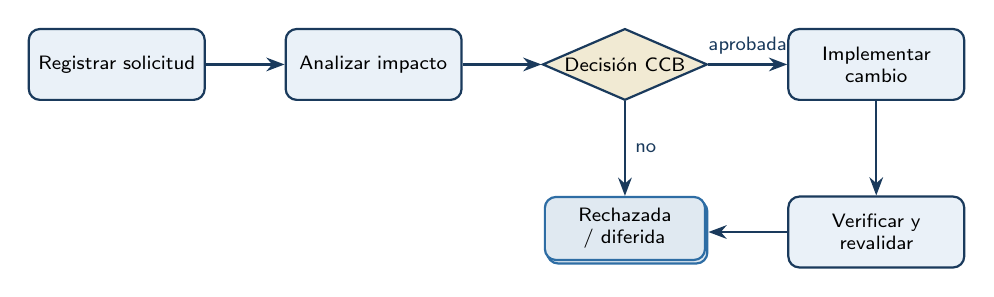
\begin{tikzpicture}[
			node distance=0.7cm and 1.0cm,
			paso/.style={draw=darkblue,thick,fill=softblue,rounded corners=4pt,minimum height=0.9cm,text width=2.0cm,align=center,font=\scriptsize\sffamily},
			ccb/.style={draw=darkblue,thick,fill=gold!25,diamond,aspect=2.3,inner sep=0pt,text width=1.7cm,align=center,font=\scriptsize\sffamily},
			fin/.style={draw=midblue,thick,fill=midblue!15,rounded corners=4pt,minimum height=0.8cm,text width=1.8cm,align=center,font=\scriptsize\sffamily},
			arr/.style={-Stealth,thick,darkblue,font=\scriptsize\sffamily}
			]
			\node[paso] (reg) {Registrar solicitud};
			\node[paso] (ana) [right=of reg] {Analizar impacto};
			\node[ccb] (dec) [right=of ana] {Decisi\'on CCB};
			\node[paso] (imp) [right=of dec] {Implementar cambio};
			\node[paso] (ver) [below=1.2cm of imp] {Verificar y revalidar};
			\node[fin] (cie) [left=of ver] {Cerrar y registrar};
			\node[fin] (rec) [below=1.2cm of dec] {Rechazada / diferida};
			\draw[arr] (reg)--(ana);
			\draw[arr] (ana)--(dec);
			\draw[arr] (dec)-- node[above]{aprobada} (imp);
			\draw[arr] (dec)-- node[right]{no} (rec);
			\draw[arr] (imp)--(ver);
			\draw[arr] (ver)--(cie);
		\end{tikzpicture}
		\caption{Proceso de control de cambios: la decisi\'on del CCB bifurca hacia la implementaci\'on o el rechazo, y todo cambio aprobado se verifica y documenta.}
		\label{fig:cambio}
	\end{figure}
	
	La documentaci\'on del cambio es tan importante como la decisi\'on misma. Cada solicitud debe registrar su origen, la justificaci\'on, el an\'alisis de impacto sobre requisitos y artefactos dependientes, la decisi\'on adoptada con su fundamento y el estado de implementaci\'on. Esta bit\'acora cumple una funci\'on doble: sostiene la rendici\'on de cuentas ---qui\'en aprob\'o qu\'e y por qu\'e--- y alimenta la trazabilidad, pues el an\'alisis de impacto solo es fiable si existen enlaces expl\'icitos entre el requisito modificado y los elementos que dependen de \'el. La norma \textit{ISO/IEC/IEEE} 29148 \citep{iso29148_2018} exige, en efecto, que los requisitos sean gestionables, propiedad que presupone un proceso de cambio documentado como el descrito.
	
	\subsection{Seguimiento y trazabilidad: tres tipos, documentaci\'on, visualizaci\'on y trazabilidad dirigida por uso}
	
	La trazabilidad es la capacidad de seguir la vida de un requisito en ambos sentidos: hacia sus or\'igenes y hacia los artefactos que se derivan de \'el. A partir de la distinci\'on seminal de Gotel y Finkelstein~\citep{gotel_finkelstein_1994} entre trazabilidad previa y posterior a la especificaci\'on, se reconocen tres tipos que la Tabla~\ref{tab:trazas} sintetiza y la Figura~\ref{fig:trazabilidad} representa: la trazabilidad hacia atr\'as, que vincula cada requisito con las fuentes que lo motivan; la trazabilidad hacia adelante, que lo conecta con el dise\~no, el c\'odigo y las pruebas; y la trazabilidad horizontal, que registra las dependencias entre requisitos.
	
	\begin{table}[htbp]
		\centering
		\caption{Los tres tipos de trazabilidad de requisitos.}
		\label{tab:trazas}
		\small\sffamily
		\begin{tabularx}{\linewidth}{@{}L{3.4cm} L{3.2cm} X@{}}
			\toprule
			\hd{Tipo} & \hd{Vincula} & \hd{Uso principal}\\
			\midrule
			Hacia atr\'as (pre-especificaci\'on) & Requisito $\rightarrow$ fuentes, interesados, normas & Justificar el porqu\'e de cada requisito y valorar cambios de origen.\\
			\rowcolor{rowgray}
			Hacia adelante (post-especificaci\'on) & Requisito $\rightarrow$ dise\~no, c\'odigo, pruebas & Comprobar cobertura e impacto de cambios sobre la soluci\'on.\\
			Horizontal (entre requisitos) & Requisito $\leftrightarrow$ requisito & Detectar dependencias, conflictos y redundancias.\\
			\bottomrule
		\end{tabularx}
	\end{table}
	
	\begin{figure}[htbp]
		\centering
		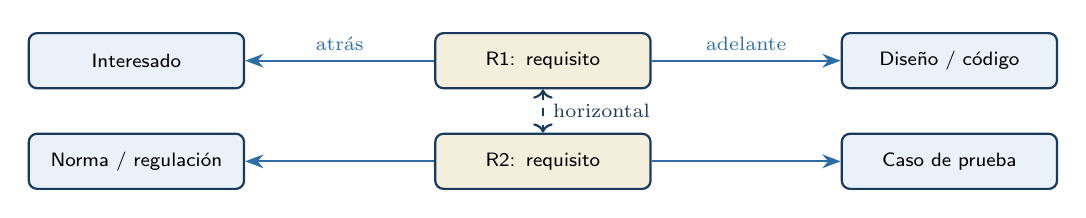
\begin{tikzpicture}[
			node distance=0.55cm,
			col/.style={draw=darkblue,thick,fill=softblue,rounded corners=3pt,minimum height=0.7cm,text width=2.5cm,align=center,font=\scriptsize\sffamily},
			reqn/.style={draw=darkblue,thick,fill=gold!20,rounded corners=3pt,minimum height=0.7cm,text width=2.5cm,align=center,font=\scriptsize\sffamily},
			arr/.style={-Stealth,thick,midblue}
			]
			\node[col] (f1) {Interesado};
			\node[col] (f2) [below=of f1] {Norma / regulaci\'on};
			\node[reqn] (r1) [right=2.4cm of f1] {R1: requisito};
			\node[reqn] (r2) [below=of r1] {R2: requisito};
			\node[col] (a1) [right=2.4cm of r1] {Dise\~no / c\'odigo};
			\node[col] (a2) [below=of a1] {Caso de prueba};
			\draw[arr] (r1) -- node[above,font=\scriptsize]{atr\'as} (f1);
			\draw[arr] (r2) -- (f2);
			\draw[arr] (r1) -- node[above,font=\scriptsize]{adelante} (a1);
			\draw[arr] (r2) -- (a2);
			\draw[<->,thick,darkblue,dashed] (r1) -- node[right,font=\scriptsize]{horizontal} (r2);
		\end{tikzpicture}
		\caption{Grafo de trazabilidad: enlaces hacia atr\'as (a fuentes), hacia adelante (a soluci\'on) y horizontales (entre requisitos).}
		\label{fig:trazabilidad}
	\end{figure}
	
	La documentaci\'on de la trazabilidad se apoya habitualmente en la \textit{matriz de trazabilidad}, que cruza requisitos con artefactos y marca cada enlace en la celda correspondiente; su lectura por filas revela requisitos hu\'erfanos sin implementaci\'on, y por columnas, artefactos sin requisito que los justifique. Para conjuntos grandes, la visualizaci\'on como grafo dirigido resulta m\'as legible que la matriz, y las herramientas CASE permiten navegar interactivamente esos enlaces. No obstante, mantener trazabilidad completa es costoso, por lo que Cleland-Huang et al.~\citep{clelandhuang_2014} proponen la \textit{trazabilidad dirigida por uso}: capturar solo los enlaces que responder\'an a preguntas concretas previstas ---an\'alisis de impacto, cobertura de pruebas, cumplimiento normativo---, de modo que el esfuerzo de trazado se justifique por su utilidad. La revisi\'on de Mucha et al.~\citep{mucha_prereq_trace_2024} confirma que la trazabilidad hacia las fuentes sigue siendo la m\'as descuidada en la pr\'actica, pese a ser la que m\'as valor aporta cuando cambian las necesidades de origen.
	
	\subsection{Requerimientos de medici\'on. Priorizaci\'on. Gesti\'on de configuraci\'on y baselines}
	
	Lo que no se mide no se puede gestionar. La medici\'on en IR observa atributos como el n\'umero de requisitos por estado, la volatilidad ---proporci\'on de requisitos modificados por unidad de tiempo---, la densidad de defectos detectados en inspecci\'on o la cobertura de trazabilidad, y usa esos indicadores para anticipar riesgos: una volatilidad alta y sostenida, por ejemplo, se\~nala que el problema a\'un no se comprende y que congelar una l\'inea base ser\'ia prematuro. La gu\'ia SWEBOK v4 \citep{swebok_v4_2024} recomienda definir cada m\'etrica a partir de la pregunta de gesti\'on que pretende responder, evitando medir por inercia.
	
	La priorizaci\'on ordena los requisitos seg\'un su valor y su urgencia para decidir qu\'e se implementa primero, decisi\'on cr\'itica cuando los recursos son limitados. La Tabla~\ref{tab:moscow} resume el m\'etodo MoSCoW, ampliamente usado tanto en contextos tradicionales como \'agiles por su simplicidad y su capacidad de forzar acuerdos expl\'icitos entre interesados \citep{wiegers_beatty_2013}.
	
	\begin{table}[htbp]
		\centering
		\caption{Categor\'ias de priorizaci\'on MoSCoW.}
		\label{tab:moscow}
		\small\sffamily
		\begin{tabularx}{\linewidth}{@{}L{3.2cm} X@{}}
			\toprule
			\hd{Categor\'ia} & \hd{Significado para la planificaci\'on}\\
			\midrule
			\textit{Must have} & Imprescindible; sin \'el la entrega carece de valor o de viabilidad legal.\\
			\rowcolor{rowgray}
			\textit{Should have} & Importante pero no vital; se incluye si el tiempo lo permite.\\
			\textit{Could have} & Deseable; primera reserva a sacrificar ante presi\'on de plazos.\\
			\rowcolor{rowgray}
			\textit{Won't have (this time)} & Fuera del alcance actual; se documenta para una entrega futura.\\
			\bottomrule
		\end{tabularx}
	\end{table}
	
	La gesti\'on de configuraci\'on cierra el ciclo al identificar de forma un\'ivoca cada versi\'on de cada artefacto y al agrupar versiones coherentes en \textit{l\'ineas base} (baselines): conjuntos de requisitos revisados y aprobados que sirven de referencia estable para el desarrollo y que solo pueden modificarse a trav\'es del proceso de control de cambios de la Subsecci\'on~4.3.2. La Figura~\ref{fig:baseline} muestra la evoluci\'on versionada de una ERS con dos l\'ineas base sucesivas. Sin este mecanismo, el equipo perder\'ia la referencia de ``qu\'e se acord\'o construir'', y la trazabilidad y las m\'etricas dejar\'ian de tener un ancla fiable.
	
	\begin{figure}[htbp]
		\centering
		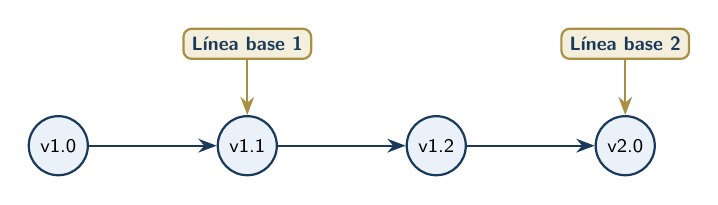
\begin{tikzpicture}[
			ver/.style={circle,draw=darkblue,thick,fill=softblue,minimum size=0.75cm,inner sep=0pt,font=\scriptsize\sffamily},
			base/.style={draw=gold!85!black,thick,fill=gold!20,rounded corners=3pt,font=\scriptsize\sffamily\bfseries,text=darkblue,inner sep=3pt},
			arr/.style={-Stealth,thick,darkblue}
			]
			\node[ver] (v0) at (0,0) {v1.0};
			\node[ver] (v1) at (2.4,0) {v1.1};
			\node[ver] (v2) at (4.8,0) {v1.2};
			\node[ver] (v3) at (7.2,0) {v2.0};
			\draw[arr] (v0)--(v1);
			\draw[arr] (v1)--(v2);
			\draw[arr] (v2)--(v3);
			\node[base] (b1) [above=0.7cm of v1] {L\'inea base 1};
			\node[base] (b2) [above=0.7cm of v3] {L\'inea base 2};
			\draw[gold!85!black,thick,-Stealth] (b1)--(v1);
			\draw[gold!85!black,thick,-Stealth] (b2)--(v3);
		\end{tikzpicture}
		\caption{Versionado de una ERS con dos l\'ineas base; cada baseline congela un conjunto aprobado modificable solo v\'ia control de cambios.}
		\label{fig:baseline}
	\end{figure}
	
	% #####################################################################
	\section{Ingenier\'ia de Requisitos en Procesos \'Agiles}
	
	Los principios de gesti\'on de la secci\'on anterior se materializan en la pr\'actica mediante herramientas de ingenier\'ia asistida por computadora (CASE) y est\'andares que fijan qu\'e propiedades debe exhibir un requisito bien gestionado. Esta secci\'on examina el instrumental de la disciplina: las herramientas que soportan la elicitaci\'on, el modelado y la gesti\'on; los est\'andares que gu\'ian su aplicaci\'on; los esquemas de atributos que hacen operativa la gesti\'on y la trazabilidad; y la gesti\'on de configuraci\'on del documento de requisitos como artefacto vivo.
	
	\subsection{Herramientas CASE para IR: Jira, Trello, Enterprise Architect, Sparx EA y ReqIF}
	
	El ecosistema de herramientas para IR abarca desde gestores ligeros de tareas hasta plataformas de modelado de nivel empresarial. Jira soporta la gesti\'on de \textit{backlogs}, historias de usuario y flujos de trabajo configurables, y domina en equipos \'agiles; Trello ofrece tableros Kanban de baja fricci\'on, adecuados para proyectos peque\~nos o para la fase inicial de organizaci\'on de ideas. En el extremo del modelado, Enterprise Architect ---producto de la empresa Sparx Systems, por lo que ``Sparx EA'' designa a la misma herramienta--- integra el modelado UML y SysML con la gesti\'on de requisitos y la trazabilidad en un repositorio \'unico. La Tabla~\ref{tab:case} sit\'ua estas herramientas seg\'un su categor\'ia y su aporte a la IR.
	
	\begin{table}[htbp]
		\centering
		\caption{Herramientas de apoyo a la ingenier\'ia de requisitos y el formato de intercambio ReqIF.}
		\label{tab:case}
		\small\sffamily
		\begin{tabularx}{\linewidth}{@{}L{3.6cm} L{3.3cm} X@{}}
			\toprule
			\hd{Herramienta} & \hd{Categor\'ia} & \hd{Aporte principal a la IR}\\
			\midrule
			Jira & Gesti\'on \'agil de trabajo & Backlog, historias de usuario, flujos y m\'etricas de avance.\\
			\rowcolor{rowgray}
			Trello & Tableros Kanban & Organizaci\'on visual ligera de requisitos y tareas.\\
			Enterprise Architect (Sparx EA) & Modelado CASE integral & Modelado UML/SysML, atributos y trazabilidad en un repositorio.\\
			\rowcolor{rowgray}
			ReqIF & Formato de intercambio & Intercambio de requisitos entre herramientas sin p\'erdida de atributos ni enlaces.\\
			\bottomrule
		\end{tabularx}
	\end{table}
	
	ReqIF merece una menci\'on aparte porque no es una herramienta sino un est\'andar de intercambio. El formato \textit{Requirements Interchange Format} de la \textit{Object Management Group} \citep{omg_reqif_2016} define una representaci\'on XML com\'un que permite transferir requisitos ---con sus atributos, valores y enlaces de trazabilidad--- entre herramientas de distintos proveedores, resolviendo el problema de la fragmentaci\'on de la cadena de suministro del software. La Figura~\ref{fig:reqif} ilustra su papel como lengua franca entre una herramienta de gesti\'on \'agil y una de modelado.
	
	\begin{figure}[htbp]
		\centering
		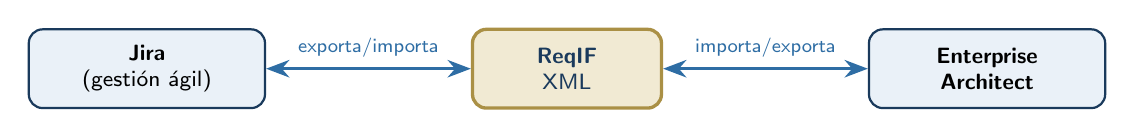
\begin{tikzpicture}[
			tool/.style={draw=darkblue,thick,fill=softblue,rounded corners=5pt,minimum width=3.0cm,minimum height=1.0cm,align=center,font=\footnotesize\sffamily\bfseries},
			hub/.style={draw=gold!85!black,very thick,fill=gold!25,rounded corners=5pt,minimum width=2.4cm,minimum height=1.0cm,align=center,font=\footnotesize\sffamily\bfseries,text=darkblue},
			arr/.style={Stealth-Stealth,very thick,midblue,font=\scriptsize\sffamily}
			]
			\node[tool] (jira) {Jira\\{\footnotesize\mdseries(gesti\'on \'agil)}};
			\node[hub] (reqif) [right=2.6cm of jira] {ReqIF\\{\footnotesize\mdseries XML}};
			\node[tool] (ea) [right=2.6cm of reqif] {Enterprise\\ Architect};
			\draw[arr] (jira) -- node[above]{exporta/importa} (reqif);
			\draw[arr] (reqif) -- node[above]{importa/exporta} (ea);
		\end{tikzpicture}
		\caption{ReqIF como formato neutral de intercambio de requisitos entre herramientas de distinto prop\'osito y proveedor.}
		\label{fig:reqif}
	\end{figure}
	
	La incorporaci\'on de inteligencia artificial a este instrumental es la tendencia m\'as reciente. Stein et al.~\citep{stein_llm_re_2026} describen c\'omo los modelos de lenguaje de gran tama\~no pueden integrarse en el proceso de requisitos para asistir en la redacci\'on, la clasificaci\'on y la detecci\'on de inconsistencias, actuando como una capa de apoyo sobre las herramientas CASE existentes en lugar de reemplazarlas. La revisi\'on de Hoy y Xu~\citep{hoy_agile_re_2023} matiza, sin embargo, que en entornos \'agiles el valor de la herramienta depende de que se integre con el flujo de trabajo del equipo, y no al rev\'es.
	
	\subsection{Est\'andares IEEE 29148:2018 e ISO/IEC 25010: aplicaci\'on pr\'actica en proyectos reales}
	
	Los est\'andares traducen los principios de la disciplina en criterios verificables. La norma \textit{ISO/IEC/IEEE} 29148:2018 \citep{iso29148_2018} fija las propiedades que debe cumplir un requisito individual ---necesario, apropiado, no ambiguo, completo, singular, factible, verificable, correcto y conforme--- y las de un conjunto de requisitos ---completo, consistente, asequible y acotado---. En la pr\'actica, estas propiedades se operacionalizan como listas de comprobaci\'on de las inspecciones de la Subsecci\'on~4.2.2: cada criterio se convierte en una pregunta que el inspector formula sobre cada requisito.
	
	Complementariamente, el modelo de calidad de producto \textit{ISO/IEC} 25010:2023 \citep{iso25010_2023} proporciona el vocabulario para especificar y validar los requisitos no funcionales. Su revisi\'on de 2023 organiza la calidad del producto en nueve caracter\'isticas ---frente a las ocho de la versi\'on de 2011---, tras a\~nadir \textit{Seguridad f\'isica} (Safety) y redefinir la antigua Usabilidad como \textit{Capacidad de interacci\'on} y la Portabilidad como \textit{Flexibilidad}. La Figura~\ref{fig:iso25010} presenta las nueve caracter\'isticas, que en un proyecto real act\'uan como una taxonom\'ia para no omitir dimensiones de calidad relevantes.
	
	\begin{figure}[htbp]
		\centering
		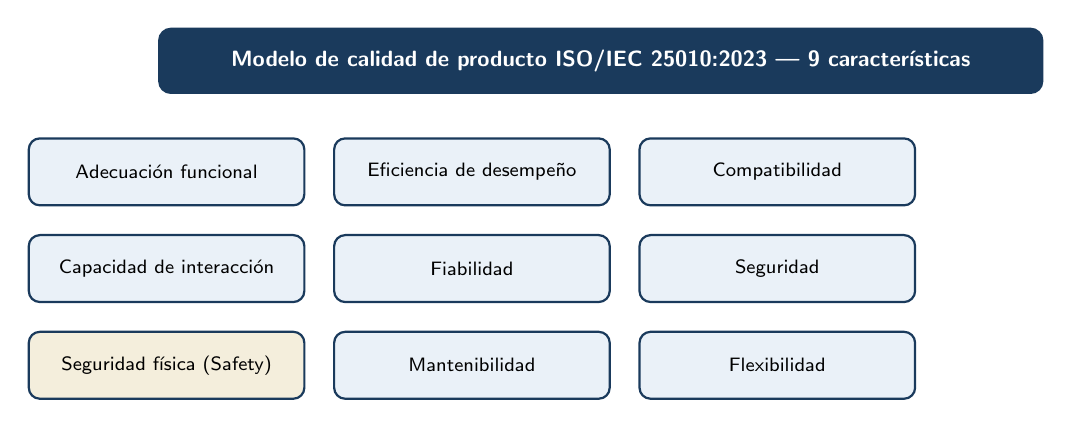
\begin{tikzpicture}[
			car/.style={draw=darkblue,thick,fill=softblue,rounded corners=4pt,minimum width=3.5cm,minimum height=0.85cm,align=center,font=\scriptsize\sffamily},
			tit/.style={draw=darkblue,very thick,fill=darkblue,text=white,rounded corners=4pt,minimum width=11.2cm,minimum height=0.8cm,align=center,font=\footnotesize\sffamily\bfseries},
			x/.style={node distance=0.35cm and 0.35cm}
			]
			\node[tit] (t) {Modelo de calidad de producto \textit{ISO/IEC} 25010:2023 --- 9 caracter\'isticas};
			\node[car] (c1) [below left=0.55cm and 3.75cm of t.south] {Adecuaci\'on funcional};
			\node[car] (c2) [right=0.35cm of c1] {Eficiencia de desempe\~no};
			\node[car] (c3) [right=0.35cm of c2] {Compatibilidad};
			\node[car] (c4) [below=0.35cm of c1] {Capacidad de interacci\'on};
			\node[car] (c5) [right=0.35cm of c4] {Fiabilidad};
			\node[car] (c6) [right=0.35cm of c5] {Seguridad};
			\node[car,fill=gold!20] (c7) [below=0.35cm of c4] {Seguridad f\'isica (Safety)};
			\node[car] (c8) [right=0.35cm of c7] {Mantenibilidad};
			\node[car] (c9) [right=0.35cm of c8] {Flexibilidad};
		\end{tikzpicture}
		\caption{Las nueve caracter\'isticas del modelo de calidad de producto \textit{ISO/IEC} 25010:2023; en gris, la incorporada en la revisi\'on de 2023.}
		\label{fig:iso25010}
	\end{figure}
	
	La aplicaci\'on conjunta de ambos est\'andares en un proyecto real sigue un patr\'on reconocible: 29148 gobierna la forma y las propiedades de los enunciados, mientras que 25010 aporta el cat\'alogo de atributos de calidad que esos enunciados deben cuantificar. As\'i, un requisito no funcional bien formado nombra una caracter\'istica de 25010, fija una m\'etrica y un umbral, y satisface los criterios de verificabilidad de 29148, de modo que pueda derivarse de \'el una prueba de aceptaci\'on no funcional como las descritas en la Subsecci\'on~4.2.4.
	
	\subsection{Atributos de requisitos para gesti\'on. Esquemas de atributos y trazabilidad en herramientas CASE}
	
	Gestionar un requisito exige tratarlo no como una frase aislada sino como un registro con atributos. Un \textit{esquema de atributos} define qu\'e informaci\'on acompa\~na a cada requisito ---identificador, prioridad, estado, fuente, estabilidad, versi\'on, m\'etodo de verificaci\'on y responsable, entre otros---, y es la estructura que las herramientas CASE materializan como campos de una ficha. La Tabla~\ref{tab:atributos} propone un esquema m\'inimo alineado con la norma \textit{ISO/IEC/IEEE} 29148 \citep{iso29148_2018} y con las recomendaciones de Wiegers y Beatty~\citep{wiegers_beatty_2013}.
	
	\begin{table}[htbp]
		\centering
		\caption{Esquema m\'inimo de atributos para la gesti\'on de un requisito.}
		\label{tab:atributos}
		\small\sffamily
		\begin{tabularx}{\linewidth}{@{}L{3.1cm} X@{}}
			\toprule
			\hd{Atributo} & \hd{Prop\'osito de gesti\'on}\\
			\midrule
			Identificador & Referencia un\'ivoca y estable para trazabilidad y control de cambios.\\
			\rowcolor{rowgray}
			Prioridad & Ordena la implementaci\'on (por ejemplo, categor\'ia MoSCoW).\\
			Estado & Situaci\'on en el ciclo de vida: propuesto, aprobado, implementado, verificado.\\
			\rowcolor{rowgray}
			Fuente & Origen del requisito, base de la trazabilidad hacia atr\'as.\\
			Estabilidad & Probabilidad de cambio; anticipa riesgo y volatilidad.\\
			\rowcolor{rowgray}
			Versi\'on & Habilita la gesti\'on de configuraci\'on y las l\'ineas base.\\
			M\'etodo de verificaci\'on & Inspecci\'on, an\'alisis, demostraci\'on o prueba; asegura verificabilidad.\\
			\bottomrule
		\end{tabularx}
	\end{table}
	
	Sobre este esquema se apoya la trazabilidad gestionada en la herramienta. Cada campo de fuente materializa un enlace hacia atr\'as, y cada v\'inculo con casos de prueba o elementos de dise\~no, uno hacia adelante, de modo que la herramienta puede computar autom\'aticamente el an\'alisis de impacto de un cambio recorriendo el grafo de la Figura~\ref{fig:trazabilidad}. La calidad de este an\'alisis depende directamente de la disciplina con que se mantengan los atributos: un estado desactualizado o una fuente omitida degradan la trazabilidad hasta volverla enga\~nosa, riesgo que la trazabilidad dirigida por uso de la Subsecci\'on~4.3.3 busca acotar concentrando el esfuerzo donde rinde.
	
	La ingenier\'ia de requisitos basada en modelos lleva este planteamiento un paso m\'as all\'a, al almacenar los requisitos y sus enlaces como elementos de un modelo formal susceptible de an\'alisis autom\'atico. La revisi\'on sistem\'atica de Zhao y Zhou~\citep{zhao_mbre_2026} evidencia que este enfoque mejora la consistencia y la trazabilidad, aunque a costa de una mayor inversi\'on inicial en la definici\'on del metamodelo y en la formaci\'on del equipo.
	
	\subsection{Gesti\'on de configuraci\'on del ERS: versiones, configuraciones y baselines de artefactos}
	
	El documento de Especificaci\'on de Requisitos de Software no es un entregable inm\'ovil sino un artefacto que evoluciona, y gestionar su configuraci\'on significa controlar esa evoluci\'on de manera reproducible. Conviene distinguir tres conceptos que suelen confundirse: la \textit{versi\'on} es un estado identificado de un \'unico artefacto en el tiempo; la \textit{configuraci\'on} es un conjunto coherente de versiones de varios artefactos que funcionan juntos ---la ERS, sus modelos UML, la matriz de trazabilidad y los casos de prueba---; y la \textit{l\'inea base} es una configuraci\'on revisada, aprobada y congelada que sirve de referencia. La Figura~\ref{fig:config} representa una configuraci\'on que agrupa versiones espec\'ificas de cuatro artefactos y se etiqueta como l\'inea base.
	
	\begin{figure}[htbp]
		\centering
		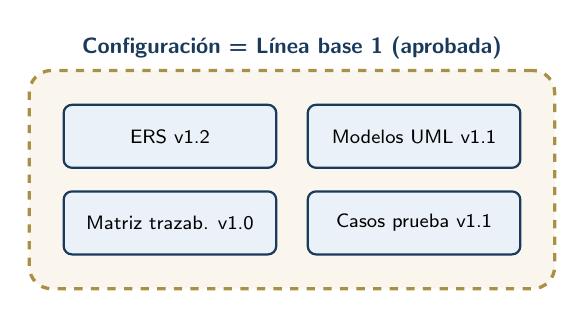
\begin{tikzpicture}[
			art/.style={draw=darkblue,thick,fill=softblue,rounded corners=3pt,minimum width=2.7cm,minimum height=0.8cm,align=center,font=\scriptsize\sffamily}
			]
			\node[art] (a1) at (0,0) {ERS v1.2};
			\node[art] (a2) at (3.1,0) {Modelos UML v1.1};
			\node[art] (a3) at (0,-1.1) {Matriz trazab. v1.0};
			\node[art] (a4) at (3.1,-1.1) {Casos prueba v1.1};
			\begin{scope}[on background layer]
				\node[draw=gold!85!black,very thick,dashed,fill=gold!10,rounded corners=8pt,
				fit=(a1)(a2)(a3)(a4),inner sep=12pt,
				label={[font=\footnotesize\sffamily\bfseries,text=darkblue]above:Configuraci\'on = L\'inea base 1 (aprobada)}] {};
			\end{scope}
		\end{tikzpicture}
		\caption{Una configuraci\'on agrupa versiones coherentes de varios artefactos; al aprobarse y congelarse se convierte en l\'inea base.}
		\label{fig:config}
	\end{figure}
	
	La gesti\'on de configuraci\'on del ERS integra as\'i todos los mecanismos del cap\'itulo. Una l\'inea base solo se modifica a trav\'es del proceso de control de cambios y su CCB (Subsecci\'on~4.3.2); cada modificaci\'on preserva la trazabilidad (Subsecci\'on~4.3.3) y actualiza los atributos de versi\'on (Subsecci\'on~4.4.3); y la comparaci\'on entre l\'ineas base sucesivas alimenta las m\'etricas de volatilidad (Subsecci\'on~4.3.4). La gu\'ia SWEBOK v4 \citep{swebok_v4_2024} subraya que esta integraci\'on es la que confiere reproducibilidad al proyecto: ante cualquier versi\'on entregada, el equipo puede reconstruir con exactitud qu\'e requisitos, modelos y pruebas la sustentaban.
	
	Cerrando el cap\'itulo, conviene notar que la validaci\'on y la gesti\'on estudiadas aqu\'i no son etapas terminales sino disciplinas transversales que acompa\~nan todo el ciclo de vida. La calidad de una ERS no se decide en un hito final de revisi\'on, sino que se construye de forma incremental mediante la validaci\'on repetida, el control disciplinado de los cambios y la trazabilidad sostenida, apoyados en est\'andares y herramientas que hacen operativos esos principios en proyectos reales.
	
	% #####################################################################
	\bibliographystyle{plainnat}
	\bibliography{referencias}
	
\end{document}